%lit. survey I
The large variety of systems and effects studied with photoelectron spectroscopy lead to diverse methods \cite{PESbook, x-ray}.
In this work the interest is in steady-state photoelectron spectra of molecular systems with a size up to some tens of atoms.
As light source a classical ultra-violet or soft X-ray source is assumed as \textit{e.g.} discharge lamps based on helium, hydrogen, mercury or similar gases.
%Hence the strength of the applied electromagnetic field is considered as weak and the kinetic energies of the outgoing electrons reach to at most tens of electron volt but can become arbitrarily small.

However, besides this scenario, in the literature a large diversity of systems, studied with different inquests using photoelectron spectroscopy, is found.
Hence a large variety of models for the description of the PES is available, differing in the numerical effort but also in the assumptions and approximations implied.
These methods can be categorised as time- and frequency-domain approaches.
{\begin{table}
\begin{small}\begin{tabular}{|c|c|c|c|c|c|}
\hline
                 &  System Size & Typical Problems & Field Str. & QC & Formalism \\
\hline
\begin{tabular}{c}Time-\\ domain  \end{tabular}    &
        \begin{tabular}{c}atomic, \\ diatomic,\\ triatomic \end{tabular} & 
        \begin{tabular}{c}HHG, \\Multiph. ionisation \end{tabular} & strong & 
        \begin{tabular}{c}(TD)DFT, \\GASCI, \\CASSCF \end{tabular} &
        \begin{tabular}{c}  Time-dep. DO \\ SE \end{tabular} \\
\hline
\begin{tabular}{c}Frequency-\\ domain \end{tabular} & 
        \begin{tabular}{c}up to \\biomolecules \end{tabular}& 
        \begin{tabular}{c} steady-state, \\ time-res. PES, \\solid states, \\... \end{tabular}& weak & 
        \begin{tabular}{c}EOM-CC,\\ RASSCF, \\TD-DFT \end{tabular}&
        \begin{tabular}{c} R-Matrix \\ DO \\Greens' Function \\ Koopmans' \end{tabular} \\
\hline
\end{tabular} \end{small}
\caption{Overview of the capabilities of time- and frequency-domain methods.}
\label{tab:PEScat}
\end{table} 
As the Table \ref{tab:PEScat} shows, the time-domain methods are restricted to small systems which is due to the fact that the $N$ electron problem needs to be solved for every time-step and hence several hundred times per simulation.
In contrast to this, frequency-domain methods require only one solution and thus are much more efficient. 
However, the neglect of the nonlinear response properties make these schemes inappropriate when multiphoton ionisation and high harmonic generation (HHG) come into play.
%These nonlinear effects however usually do not play any role for classical light sources such as gas discharge or heat lamps and even most non-pulsed lasers.

Among the the frequency domain methods, the most prominent representative is the method denoted as Koopmans' approach in Table \ref{tab:PEScat} \cite{Koerzd1,PottsHolland,dos,dos2}.
In this scheme, the systems ground state is computed with a given quantum mechanical method to obtain the electronic binding energies.
The photoelectron spectrum is than estimated using the orbital energies as the transition energies and using uniform intensities.
While this method has shown to be at qualitatively in good agreement with experiment for some systems \cite{Koerzd1,Koerzd2, EggerKronik,PottsHolland,YepesJaque}, 
it breaks down in cases of strong electron correlation \cite{2phcederbaum,2phcederbaum2} due to strong changes in the orbitals upon ionisation.
%Since the estimation of the role of correlation effects can only hardly be estimated in advance, this method has only poor predictive character.
This method is characterised by its low computational costs and robustness and thus well-suited for very large systems such as solid states where calculations beyond ground-state DFT are very demanding on not feasible at all.

\begin{wrapfigure}{r}{0.7\textwidth}
   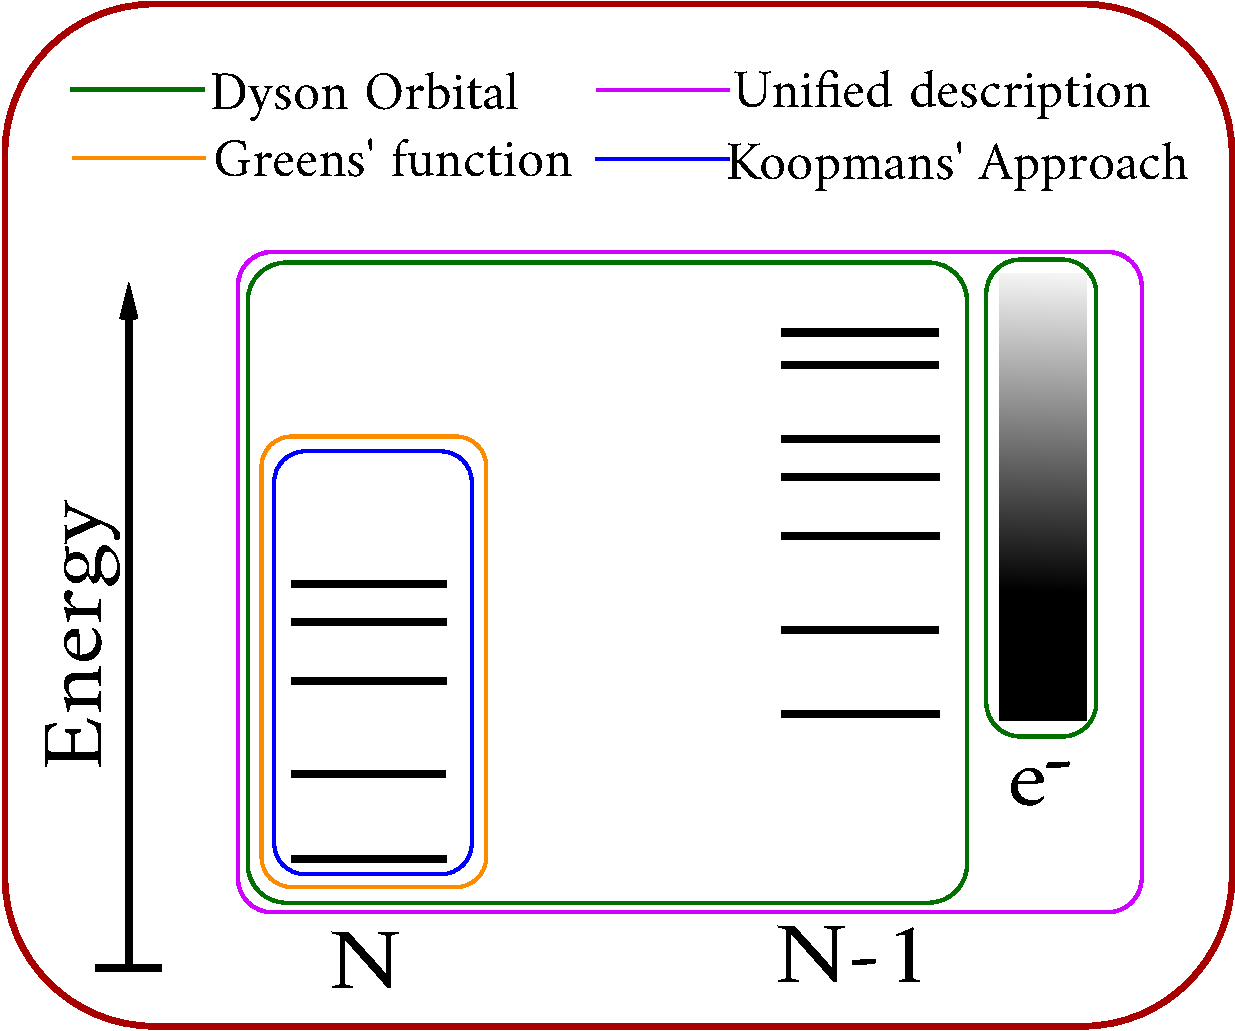
\includegraphics[width=0.7\textwidth]{Figures/Methods}
   \caption{Scheme of the system-representation used in the different methods.}
   \label{fig:PEScat}
\end{wrapfigure}
While in the Koopmans' approach only the ground state of the un\-ion\-ised state is considered, other methods treat the system under study in different ways.
In Figure \ref{fig:PEScat} the model of the system used the most important methods is schown schematically.
In a similar way as the Koopmans' theorem takes only the initial state into account, the Greens' function approach is implicit on the photoelectron.
A short introduction to this approach is given in section \ref{ch:gf}.
Among those methods that treat all $N$ electrons both in the initial and final state is a large group of methods where the photoelectron is treated on the same footing.
Out of this class, several approaches both in time- and frequency-domain are described in section \ref{ch:r-mat}.
Finally the Dyson orbital formalism describes the full $N$-electron system in the final state but here the photoelectron is treated separately, neglecting correlation effects with the bound states.
A more detailed derivation of the expressions used in this formalism is given in section \ref{ch:do}.

\section{The Greens' Function Approach}
\label{ch:gf}
In contrast to most other quantum-chemical methods, in the Greens' function approach expectation values for a given operator $\hat{O}$ are not computed as a scalar product $\langle \Psi^N |\hat{O} | \Psi^N \rangle $ with the wave function $|\Psi^N\rangle$ of the $N$ electron state of interest, but by contour integrals with the Greens' function \cite{bookGF, 1pGFcederbaum}.
Thereby the (one particle) Greens' function is a matrix $\mat{G}$ whose elements are defined as
\begin{equation} \label{eq:defGF}
G_{j,k}(t,t')= -\text{i}\langle \Psi^N | \hat{T}\left(\hat{a}_j(t)\hat{a}_k^\dagger(t')\right)|\Psi^N\rangle 
\end{equation}
with the creation operator $\hat{a}^\dagger_j (t)=e^{\text{i}\hat{H}t}\hat{a}^\dagger_j e^{-\text{i}\hat{H}t}$ of an electron in state $j$ at time $t$ in Heisenberg picture and the annihilation operator $\hat{a}(t)=e^{-\text{i}\hat{H}t}\hat{a}_j e^{\text{i}\hat{H}t}$ respectively.
$\hat{T}$ denotes is the Dyson time ordering operator that orders the operators $\hat{a}$ and $\hat{a}^\dagger$ by their time arguments to ensure that the operator with smaller time argument is on the right hand side of the other one \cite{bookGF}.
Hence, the Greens' function can be interpreted as an additional electron (or hole, depending on the time ordering) propagating from $t'$ to $t$ in a system described by the Hamiltonian $\hat{H}$ \cite{bookGF}.

In this approach the calculation of photoelectron spectra is formulated such that the poles and residues of the Fourier transformed Greens' function are searched.
This becomes clear when writing the time-ordering operator in equation (\ref{eq:defGF}) explicitly
\begin{equation} \label{eq:GF}
G_{j,k}(t,t')= -\text{i}\langle \Psi^N | \hat{a}_j(t)\hat{a}^\dagger_k(t') |\Psi^N\rangle \Theta(t-t') -
                   \text{i} \langle \Psi^N | \hat{a}^\dagger_k(t')\hat{a}_j(t) |\Psi^N\rangle \Theta(t'-t).
\end{equation}
Inserting the closure relation $\hat{1}=\sum_k |\Psi^M_k\rangle\langle \Psi^M_k |$, where $M=N\pm 1$ and $|\Psi^M_k\rangle$ describes a bound state, between the operators in both terms of (\ref{eq:GF}) the Lehmann representation \cite{bookGF} is obtained whose Fourier transform is
\begin{equation}\label{eq:gfSpect}
G_{j,k}(\omega)=-\text{i} \sum_k\frac{\left|\langle \Psi^N | \hat{a}_j|\Psi^{N+1}_k \rangle \right|^3}{\omega-(E_k^{N+1}-E^N)+\text{i}\nu}-
                \text{i}\sum_k\frac{\left|\langle \Psi^N | \hat{a}^\dagger_k|\Psi^{N-1}_k \rangle \right|^2}{\omega+(E_k^{N-1}-E^N)-\text{i}\nu},
\end{equation}
where $\nu$ is a small parameter arising from calculation of principal value.
Further $\omega$ denotes the argument of the Fourier transform while $E^N$ and $E_k^M$ are the energies of the $N$-electron ground stated $|\Psi^N\rangle$ and of the $k$-th $M$-electron state $|\Psi_k^M\rangle$ respectively.
In this form, the second sum corresponds to transitions in the photoelectron spectrum: the nodes of the denominator (poles of the Greens' function) can be easily assigned to the ionisation potentials and thus the transition energies in photoelectron spectra.
Further, the integrals in the nominator are equivalent to the sudden approximation derived in chapter \ref{ch:sa} and hence provide a good approximation to the transition strengths.
The terms in the first sum correspond to the respective quantities of electron detachment \cite{1pGFcederbaum}.

However, computing the Greens' function is a demanding task which is of similar complexity as the computation of a solution to the SE.
Over the years several approaches were developed of which the algebraic diagrammatic construction \cite{1pGFcederbaum} and the equation of motion \cite{PottsHolland,1pGFcederbaum} are the most prominent.
In the diagrammatic construction one starts with an initial zeroth order Greens' function $\mat{G}^0(\omega)$ constructed in a Hartree-Fock basis and corrects it iteratively by $\mat{G}^0(\omega)\mat{\Sigma}(\omega)\mat{G}(\omega)$, where $\mat{\Sigma}(\omega)$ is the self-energy, an effective potential that is used to recover electron correlation and relaxation effects \cite{GreenBayse}.
The self-energy usually is expanded in a perturbation series with respect to Feynman diagrams with increasing number of vertices and is exact in the limit of infinite terms \cite{bookGF,cederbADC}.
The one-particle energies, Coulomb matrix elements and overlap integrals are obtained from self-consistent field (SCF) calculations \cite{1pGFcederbaum} which are usually obtained on the HF-level \cite{GreenBayse} but (TD)DFT or any other quantum chemical method can be used as well \cite{Koerzd1}.
While being much easier to compute, the Hartree-Fock basis has the disadvantage that only single configurational electronic states can be treated.

On the other hand, an important advantage of the Greens' function method is that the transition energies are computed directly while in most other methods calculated it as the difference of the initial and final state functions.
The latter approach however can lead to errors in the electron volt range when the interaction energies are badly estimated \cite{1pGFcederbaum}.

%Another, yet similarly simple approach used in cases where only few electronic transitions are present is to fit the intensity to experimental data \cite{winterWater,hemberg1}.
%This is especially used when the vibrational structure is resolved.
%
%Here, two different approaches are possible.
%While most methods use Fermis Golden Rule 
%\[  \sigma(\omega)\propto |\langle |\hat{mu}|\rangle|^2 g(E_f-E_i+h\nu -\omega)
%\]
%where the intensity of the transitions is calculated via the dipole matrix elements, the other route is
%via the complex polarisability $\alpha(\omega)=\int_{IP}^\infty \frac{df(\epsilon)}{\epsilon^2-\omega^2}$. 
%In the latter case, the spectrum is obtained via
%\[ \sigma(\omega)=\frac{4\pi \omega}{c} Im(\alpha(\omega)).\]
% Some of them are especially generated for special geometries such as the R-matrix method described in chapter \ref{ch:r-mat}, others such as the Greens' function or Dyson orbital formalism introduced in the chapters \ref{ch:gf} and \ref{ch:do} respectively are more general but can not reach the same accuracy.
% Besides different classes of molecules, also the light irradiation considered can differ: Some methods are especially designed for large intensities \textcolor{green}{sources} or kinetic energies in the relativistic regime \textcolor{green}{source}.
 %In this work, however, only methods applicable in more moderate regimes are considered, meaning that perturbation theory is applicable and the kinetic energy of the photoelectron is considered to not above the $keV$-range.
%\section{Methods where electron is treated in same footing as bound states}
%\section{Methods with Unified Description of Bound and Free States}
\section{Combined Bound and Continuum State Representation}
\label{ch:r-mat}
%Another large class of methods for computing photoelectron spectra uses perturbation theory in frequency domain or the dipole autocorrelation function in time domain respectively.
%In frequency domain thereby the initial state and final state are described therein each as $N$ electron systems with a uniform scheme, requiring the basis set to be formulated general enough to represent bound as well as free states.
In contrast to the Greens' function method in which the explicit description of the FEF  omitted, a large group of methods describes the full $N$-electron system before and after the ionisation respectively.
With this approach electron correlation effects also between bound and unbound states are accounted for but a large and flexible basis is required which can represent bound as well as unbound states of electrons.
Due to this, these methods are generally restricted to small systems that fulfil certain symmetry-requirements and have only a low amount of electrons.

The most prominent representative of this class in frequency-domain is the R-matrix method \cite{r-mat, r-mat2,Burke}.
Its general idea is to conduct a partition of space into regions which are treated differently, connected by explicit boundary conditions to ensure smoothness of the wave function.
These regions are constructed with concentric spheres, restricting the symmetry of wave functions in this scheme.
Nonetheless it is applied not only to atoms \cite{Li-R,Li-R1,Li-R2} but also to small molecules \cite{R-mol1,R-mol2}.
\begin{wrapfigure}{r}{0.48\textwidth}
   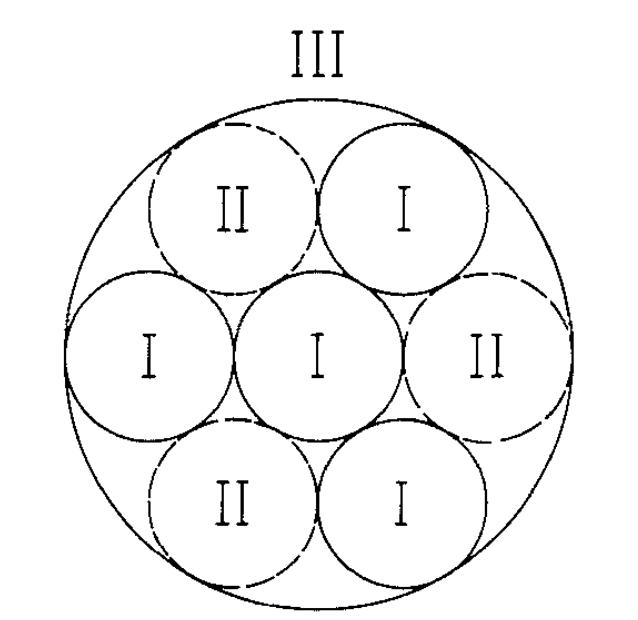
\includegraphics[width=0.48\textwidth]{Figures/JohnsonSpheres}
   \caption{Schematic view of the space partition scheme used by Johnson for a four-atomic molecule:
    I: atomic, II: interatomic and III: extra-molecular space \cite{johnson}.}
   \label{fig:johnson}
\end{wrapfigure}
In the R-matrix formalism the inner region is chosen large enough to contain the bound part of the $N$-electron function that is usually represented by a configuration interaction (CI) expansion of Slater determinants (SDs), using a with a linear combination of atomic orbitals (LCAO) basis or a grid representation \cite{Burke}.
The FEF commonly is described by a linear combination of bound orbital type functions and continuum functions such as Coulomb waves \cite{r-mat, r-mat2}. %or a product description of spherical Harmonic and a spline-based radial function.
%a antisymmetrised product of Coulomb type wave function with ...\cite{r-mat,r-mat2}.
In the outer region, an expansion in Coulomb waves is used to ensure the asymptotically correct behaviour.
In addition to the inner region, where correlation plays an important role, and the asymptotic outer region further intermediate regions can be added  where the FEF is represented by a multipole-radiation expansion which is a polynomial of inverse powers of the distance to the centre \cite{Burke}.

%in which the multipole functions can be added\cite{Burke}.
A generalisation to non-spherical systems is employed, \textit{e.g.}, by Johnson \cite{johnson} who used different kinds of non-concentric spheres.
One set of spheres is centred each at an atom while others are placed such in the interatomic regions such that the space is filled as dense as possible as shown in Figure \ref{fig:johnson} for a molecule with four atoms.
Each atom is located in the centre of a circle denoted as I while the circles II fill the interatomic space.
An outer sphere surrounds the molecule to account for the asymptotic region similar to that used in R-matrix theory.
In this scheme the exchange-correlation is treated on an approximate level \cite{slaterJohn} and is spherically averaged, resulting in a description that is equivalent to the muffin-tin potential which is a well-known model in solid state physics \cite{MufTin,MufTin1}.
The continuity of the wave-functions as well as their derivatives is a ensured over the regions using multiple-scattered-wave theory \cite{johnson}.
%Thereby the potential energy contains besides the Coulomb term also a statistical approximation of the exchange correlation of the form
%\begin{equation}
 %V_{x\alpha}(\vec{r}) = -6\alpha\left( \frac 38 \pi \rho(\vec{r})\right)^{\frac 13} 
%\end{equation}
%where $\rho(\vec{r})$ is the electron density and $\alpha$ is a parameter that is chosen differently for each element.
%In each of the regions the potential %energy is expanded in a superposition of spherical harmonics that is truncated after the $l=0$ term which is equivalent to the muffin-tin potential which is well-known especially for solids \cite{MufTin,MufTin1}.
The wave-functions are chosen in each region as a one-centre expansion of the form
\begin{equation} \label{eq:radSE}
\Psi(\vec{r})=\sum_{l=2}^{l_\text{max}}\sum_{m=-l}^l c_{l,m} R_l(r) Y_l^m(\theta, \phi)
\end{equation}
where $r,\theta,\phi$ are the coordinates of the spherical coordinate system and $Y_l^m(\theta,\phi)$ are the spherical Harmonics \cite{Lifschitz}.
The radial function $R_l(r)$ solves the radial SE 
\begin{equation}
\frac{\partial^2 R(r)}{\partial r^2} + \left( E-V(r) + \frac{l(l+1)}{r^2} \right)R(r)=0
\end{equation}
with the respective spherically averaged potential $V(r)$ \cite{johnson}.

%A similar approach is to describe the bound and free states at the same level as applied by DeCleva \textit{et al.}  $H_2^+$\cite{H2pDeCleva}.
An approach applied by DeCleva \textit{et al.} to $H_2^+$ \cite{H2pDeCleva} and benzene \cite{DeClevaBenzene} resigns the use of spheres, allowing for more general boundaries between the inner and outer regions.
Here the FEFs are globally described in the one-centre expansion (\ref{eq:radSE}) where $R(r)$ is described by a B-spline basis. % (details about the spline description are given in section \ref{ch:dvr}).
The advantage of the spline-based description is that smoothness at the interface of the regions is ensured intrinsically.

Another scheme in frequency domain is used by Richards and Larkins \cite{richardsFD} with a hybrid ansatz: While the bound states of the H$_2$ molecule are described in the common LCAO scheme, the FEF is described by the product ansatz $\Psi(\vec{r}) = R(r,\theta) e^{im\phi}$ where $R(r,\theta)$ is obtained on a two-dimensional grid using a finite difference (FD) scheme.
In contrast to the previously described methods, here no partition of space is conducted but instead a finite box with Dirichlet boundary conditions is used.
Moreover, the FEF is treated on the HF-level, neglecting correlation effects \cite{richardsFD}.

Similar descriptions are used in time-domain by several authors \cite{CAPccEOM, bauch1, taoDVR}.
Since a time-domain description requires the recomputation of the $N$-electron function for each time-step and thus several hundreds to thousands of times per simulation, its computational effort is increased by far.
On the other hand, time-domain methods allow the description of non-linear effects such as high harmonic generation and multi-photon ionisation \cite{as2} which are both not perceptible by frequency-domain methods.

An important difference between time- and frequency-domain methods of practical means is that in time-domain free particles are described by a wave packet and hence as a localised function.
Moreover, at short times after ionisation the continuum states often can be assumed to be coupled diabatically to the bound states (\textit{i.e.} the wave packet does not move away from the ionic remainder).
Under this assumption, the spacial part of the FEF can be written as a linear combination of bound state functions but having a complex energy that determines the oscillations and finite lifetime of the function \cite{CAPccEOM}.
Moreover a complex absorbing potential (CAP) (discussed in chapter \ref{ch:cap} in more detail) is most often applied, ensuring the assumption of diabatic coupling to the bound states by cutting off that part of the wave function which is not localised at the molecule anymore.
Due to these considerations the LCAO basis can be used here for the description of the free particles as well, as conducted \textit{e.g.} by Jagau \textit{et al.} \cite{CAPccEOM}.
In other simulations, grid-based descriptions are chosen using symmetry-adapted coordinate systems \cite{radau,jacobi, hyperspheric,taoDVR}, allowing a product ansatz and hence a reduction in dimensionality.
%In other simulations, a grid-based description is chosen using spherical, elliptical or hyperspherical coordinates, allowing ng for a product ansatz and hence a reduction to one dimension.
On the remaining one-dimensional grids often a discrete variable representation (DVR) (described in section \ref{ch:dvr} of this thesis) is chosen.
As an example, Yip \textit{et al.} \cite{yipDVR} simulate double ionisation of atomic beryllium in spherical coordinates, using the expansion (\ref{eq:radSE}) where $R(r)$ is separated into two regions in which a DVR and a finite element DVR (FE-DVR) scheme are used respectively.
Tao \textit{et al.} \cite{taoDVR} as well as Bauch \textit{et al.} \cite{bauch1, bauch2} use the FE-DVR basis in spheroidal coordinates respectively.

\textcolor{red}{This is by far not a complete list; are these at least the most important methods?}

%A different technique is used by Son \textit{et al.} who use time dependent density functional theory (TDDFT) based on a finite volume scheme instead of the usual LCAO approach.
%Thereby no asymptotic region is utilised, instead the region of interest is chosen by setting a sphere with a given radius around each atom \cite{Son_Chu0,Son_Chu}.

%Sato \textit{et al.}\textcolor{green}{sources} 
\section{The Dyson Orbital Formalism}
\label{ch:do}
The Dyson orbital (DO) formalism can be considered as an approximation to the formalisms described above where the free and bound states are described separately.
Using such a separation leads to an neglect of correlation effects between the outgoing electron and the bound states and is often denoted as sudden ionisation limit \cite{ezDyson,MAgg}.
In this formalism the overlap between the initial state and the bound part of the final state is formulated as an effective one-electron quantity, called DO.
%reducing the computation of the dipole matrix elements to a one-electron integration.
Usually the DO scheme is considered in the frequency domain, but a time domain formulation exists as well and is described in the following subsection \cite{TD-do}.
%The DO therein can be interpreted as a quasi-particle that is removed from the molecules; incorporating multi-particle effects such as electron relaxation or instantaneous excitation of other electrons.

\subsection{Time-dependent Dyson Orbitals}
%There are several approaches towards Dyson orbitals.
%Here we will mainly follow the derivation of Gritsenko \textit{et al.} \cite{TD-do}, starting from an exact time-dependent expression.
%Here we will mainly follow the derivation of Gritsenko \textit{et al.} \cite{TD-do}, starting from an exact time-dependent expression.
%Thereby the $j$-th time dependent Dyson orbital (TDDO) is defined as the overlap integral of the $j$-th final ionised state $\Psi_j^{N-1}^\dagger(\vec{r}_2,\hdots,\vec{r}_N)$ with the unionised initial $N$-electron state $\Psi^{N}(\vec{r}, \vec{r}_2,\hdots,\vec{r}_N)$
%\begin{equation}
%\Psi_\text{DO}^j(\vec{r}) = \sqrt{N} \int \Psi_j^{N-1}^\dagger(\vec{r}_2,\hdots,\vec{r}_N)
%                                           \Psi^{N}(\vec{r}, \vec{r}_2,\hdots,\vec{r}_N)
%                            d\vec{r}_2 \hdots d\vec{r}_N .
%\end{equation} 
A good starting point for the DO formalism is an expansion of the time-dependent $N$-electron function $\Psi^N(\vec{r}, \vec{r}_2, \hdots,\vec{r}_N, t)$ in the form
\begin{equation} \label{eq:DOexpansion}
%\Psi^N(\vec{r}, \vec{r}_2, \hdots,\vec{r}_N, t)=\frac{1}{\sqrt{N}} \sum_k \Psi^k_\text{DO}(\vec{r},t) \Psi_k^{N-1}(\vec{r}_2, \hdots,\vec{r}_N)e^{\text{i}E_k^{N-1}t}
| \Psi^N (t)\rangle =\frac{1}{\sqrt{N}} \sum_k |\Psi_k^{DO}(t)\rangle | \Psi^{N-1}_k \rangle e^{iE_k^{N-1}t}
\end{equation}
where $E_k^{N-1}$ are the energies of the $N-1$-electron bound states described by the wave functions $|\Psi_k^{N-1}\rangle$ that are complete in the space of $N-1$-electron wave-functions.
The expansion coefficients $|\Psi_k^{DO}(t)\rangle$ have the dimensionality of a one-particle function and are denoted as the time-dependent DO (TDDO).
An important feature of the expansion (\ref{eq:DOexpansion}) is that the dynamics of the $N$-electron system are reduced to a system of one-electron quantities $|\Psi_k^\text{DO}(t)\rangle$ propagated by a TDDFT-like equation of motion \cite{TD-do}.
\textcolor{red}{Put the EOM here?}
%\begin{equation}
%\text{i}\frac{\partial}{\partial t}|\Psi_j(t)\rangle =
%\left{-\frac 12 \nabla^2 + \hat{v}_\text{ext}(\ver{r},t) +\Delta_j(t) \right} |Psi_j(t)\rangle
%\end{equation}
In this approach the interaction of the DO with the bound states is approximated by the mean-field electrostatic potential \cite{TD-do}, neglecting exchange and correlation.

The physical interpretation of the DO becomes clear when regarding its definition, given by
\begin{equation} \label{eq:TDDO}
%\Psi^k_\text{DO}(\vec{r},t) = \sqrt{N} \int \Psi_k^{N-1 \dagger}(\vec{r}_2,\hdots,\vec{r}_N) e^{\text{i}E_k^{N-1}t}
                              %\Psi^N(\vec{r}, \vec{r}_2, \hdots,\vec{r}_N, t) d\vec{r}_2,\hdots d\vec{r}_N.
|\Psi_k^\text{DO}(t)\rangle =  e^{\text{i}E_k^{N-1}t}\sqrt{N} \langle \Psi_k^{N-1} |\Psi^N(t) \rangle.
\end{equation}
The remaining coordinates not integrated in (\ref{eq:TDDO}) belong to the photoelectron since $|\Psi^{N-1}(t)\rangle$ is restricted to the description of bound states
Hence in a frozen orbital approximation the DO is identical to the photoelectron.
However, relaxation-effects change the overlap and thus lead to additional contributions to the TDDO.
These considerations suggest to interpret the TDDO as a quasi-particle describing the electron that is ionised, including relaxation and correlation effects \cite{ezDyson,TD-do}.
%Thereby especially three time slices are interesting: $t<0$ \textit{i.e.} before the ionisation , $t=0$ and the limit of $t\rightarrow \infty$.
%For $t<0$ hence the expression (\ref{eq:DOexpansion}) describes the unionised system in its initial state where the DO is a molecular orbital and equation (\ref{eq:DOexpansion}) is a way to write a Slater determinant (SD).
%In the limes of $t\longrightarrow \infty$ thereby $|\Psi_k^{N-1}\rangle$ describes the ionic remainder in a state $k$ and hence the TDDO is the free electron function (FEF) whose energy is determined by the laser pulse which ionised the system as well as the energy $E_k^{N-1}$.
%However, due to relaxation and correlation effects, the orbitals in the final states are different from those in the $N$ electron state and hence these changes are also contained in the TDDO.
%For the case $t=0$ these relaxation effects also are included in the TDDO but the FEF did not change its wave function with respect to the ionised orbital hence its wave function is that of the removed electron, amended by combination and relaxation effects. \\ \\
%Thereby, this formalism resolves two main problems of time propagation using standard TDDFT which are the missing memory effects due to an approximate exchange potential that depends on the current density only. % this is resolved because in the 1-particle EOMs only static electron-electron interaction potentials occur.
%The second problem often occurring is that usual TDDFT is not able to predict correlated multiple ionisations which can be resolved with this formalism as well \cite{TD-do}.

\subsection{Time-independent Dyson Orbitals}
Working in frequency domain, no propagation of the TDDO nor the ionised system (\ref{eq:DOexpansion}) needs to be considered.
The time-independent DO is defined rather as the TDDO at $t=0$.
Since at this point the FEF is coupled adiabatically to the respective orbitals, the DO can be interpreted as quasi-particle that is ejected by the irradiating light \cite{ezDyson}.

%To see the benefit of using the DO formalism for computing photoelectron spectra, we start with the photoelectron cross section in atomic units
The main advantage of this formalism in frequency-domain becomes clear when the photoelectron cross-section is considered.
In the Fermis' Golden Rule formulation, which assumes the wavelength to be much larger than the system under study and weak irradiating light-field, the cross-section is in atomic units \cite{richardsFD,MAgg}
\begin{equation} \label{eq:sigma}
\sigma(\epsilon) =\frac 23
           \nu \sum_k\left| \langle \Psi^N_i | \vec{\hat{d}} | \Psi^N_{k}\rangle
\right|^2  
             \propto \sum_k \left|  \vec{D}_k \right| ^2
\end{equation}
where $\epsilon=\nu-(E_k-E_i)$ is the kinetic energy of the photoelectron that is determined by the photon energy $\nu$ and the energies $E_i$ of the initial unionised state $|\Psi^N_i \rangle$ and the total binding energy $E_k$ of the final ionised state $|\Psi^N_k\rangle$ which includes all electrons.
Writing the initial and final states each as SDs
\begin{subequations} \label{eq:SDs} \begin{align}
   |\Psi^N_i\rangle &= \hat{A}_N | \Phi_{i,1} \hdots \Phi_{i,N} \rangle \\
   |\Psi^N_k \rangle &= \hat{A}_N | \Phi_{k,1}\hdots \Phi_{k,N-1} \Psi_k^\text{el} \rangle
\end{align}\end{subequations}
where $\hat{A}_N$ is an $N$-electron antisymmetrisation operator.
Furthermore the one-electron quantities $|\Phi_{k,j}\rangle$ denote the $j$-th (Kohn-Sham) orbitals and $\Psi_k^\text{el}$ is the FEF.
The index $k$ enumerates the final states which can have an arbitrary electron configuration here.
The dipole operator $\hat{\vec{d}}$ is a one-electron operator that can be written as$\hat{\vec{d}}=\sum_{j=1}^N \hat{\vec{d}}_j$ where $\hat{\vec{d}}_j=\vec{r}_j$ in length gauge or $\hat{\vec{d}}_j=\nabla_j/(2\pi\nu)^2$ in velocity gauge respectively \cite{richardsFD}.

Using the SD representations (\ref{eq:SDs}), the integral $\vec{D}_k$ in equation (\ref{eq:sigma}) can be written as
\begin{equation} \label{eq:derDO1}
\vec{D}_k = \langle
\Phi_{i,1}  \hdots\Phi_{i,N} | \hat{A}_N \sum_{j=1}^N\hat{\vec{d}}_j \hat{A}_N |
\Phi_{k,1}\hdots\Phi_{k,N-1} \Psi_\text{el} 
\rangle 
\end{equation}
where hermiticity of the antisymmetrisation operator is used.
The expression (\ref{eq:derDO1}) can be further expanded by commuting $\hat{A}_N$ with the dipole operator and making use of the relation $\hat{A}_N\hat{A}_N=\sqrt{N!}\hat{A}_N=\sum_P (-1)^p \hat{P}$ where the sum goes over all permutations $\hat{P}$ with parity $p$
\begin{align} \label{eq:derDO2}
\vec{D}_k & = \sqrt{N!}\sum_P (-1)^p \sum_{j=1}^N \langle
\Phi_{i,P(1)}\hdots\Phi_{i,P(N)} |\hat{\vec{d}}_j |
\Phi_{k,1}\hdots\Phi_{k,N-1} \Psi_\text{el}  \rangle  \\
  & = \sqrt{N!}\sum_P (-1)^p \sum_{j=1}^N 
  \langle \Phi_{i,P(j)} | \hat{\vec{d}}_j | \Phi_{k,j} \rangle
          \langle \Phi_{i,P(1)}  |\Phi_{k,1}   \rangle
  \hdots  \langle \Phi_{i,P(j-1)}|\Phi_{k,j-1} \rangle \\
  & \times\langle \Phi_{i,P(j+1)}|\Phi_{k,j+1} \rangle
          \langle \Phi_{i,P(N-1)}|\Phi_{k,N-1} \rangle
  \hdots  \langle \Phi_{i,P(N)}  |\Psi_\text{el}\rangle 
\end{align}
where $P(j)$ is a permutation of the $j$-th orbital.
Thereby the term $j=N$ differs qualitatively from the others since the dipole operator acts on the FEF.
Hence the sum can be reordered to obtain
\begin{align} \label{eq:fullDO}
  \vec{D}_k & = 
  \underbrace{\sqrt{N!}\sum_P (-1)^p 
          \langle \Phi_{i,P(1)}  |\Phi_{k,1}    \rangle
  \hdots  \langle \Phi_{i,P(N-1)}|\Phi_{k,N-1}  \rangle
  \langle \Phi_{i,P(N)} }_{\langle \Psi_k^\text{DO}|} | \hat{\vec{d}}_j | \Psi_\text{el} \rangle + \nonumber \\
  & 
       \sqrt{N!}\sum_P (-1)^p \sum_{j=1}^{N-1} 
          \langle \Phi_{i,P(1)}  |\Phi_{k,1}    \rangle
  \hdots  \langle \Phi_{i,P(j-1)}|\Phi_{k,j-1}  \rangle \times \nonumber \\
  &       \langle \Phi_{i,P(j+1)}|\Phi_{k,j+1}  \rangle
  \hdots  \langle \Phi_{i,P(N-1)}|\Phi_{k,N-1}  \rangle
 \langle \Phi_{i,P(j)}|\hat{\vec{d}}_j |\Phi_{k,j}\rangle
  \langle \Phi_{i,P(N)}| \Psi_k^\text{el} \rangle
\end{align}
where the first sum is denoted as DO and the second as conjugate DO respectively \cite{saPonzi}.
To reduce the large amount of integrals therein, the strong orthogonality approximation is applied under the assumption that the overlap 
\begin{equation}
 \langle \Phi_{k,j}  |\Psi_\text{el}\rangle=0 \quad \forall\, j=1,\hdots, N.
\end{equation}
of the FEF with all bound states vanishes.
This would be strictly valid if they would correspond to the same Hamiltonian.
But in most cases the orbitals of the ionised and unionised state are similar, leading to small but non-zero overlaps \cite{saPonzi,GrellKuehn}.
Applying the strong orthogonality condition leads to the drop out of the second sum in equation \ref{eq:fullDO} and the transition dipole moment simplifies to
\begin{align} \label{eq:sigma_do}
\vec{D}_k&= \sum_p (-1)^P \langle \Phi_{i,P(1)}  |\Phi_{k,1} \rangle
            \hdots  \langle \Phi_{i,P(N-1)}|\Phi_{k,N-1} \rangle
                   \langle \Phi_{i,P(N)} |\hat{\vec{d}}_j |\Psi_k^\text{el}\rangle \nonumber \\
    &= \langle \Psi_k^\text{DO}| \hat{\vec{d}}_j| \Psi_k^\text{el}\rangle
\end{align}
which corresponds to the definition of the TDDO in equation (\ref{eq:TDDO}) for $t=0$ as mentioned above.
The expression for the PES cross-section in the DO formalism simplifies to
%Though the cross section simplifies from the $N$ electron expression (\ref{eq:sigma}) to 
\begin{equation} \label{eq:DO_pes}
\sigma(\epsilon) =\frac 23 (\epsilon +E_k-E_i)
           \sum_k \left|  \langle \Psi^k_\text{DO} | \hat{\vec{d}} | \Psi_\text{el}\rangle  \right|^2 .
\end{equation}
In the derivation given here, it is assumed that initial and final state can be represented by a single SD each.
In practice, often states are described by a linear combination of SDs with different electron configurations.
A respective generalisation of the DO is straight forward but introduces additional summations and thus leads to more complex terms.

\subsection{Sudden Approximation}
\label{ch:sa}
Further simplification of the DO formalism can be obtained by applying the so-called sudden approximation (SA) where the computation of the FEF is avoided.
In the SA it is assumed that the transition to a continuum function with corresponding energy has a constant probability which can be justified by the high degree of degeneracy of continuum functions for each given energy.
Thus, the transition probability
\begin{equation}
\vec{D}_k= \sum_p (-1)^P \langle \Phi_{i,P(1)}  |\Phi_{k,1} \rangle
           \hdots  \langle \Phi_{i,P(N-1)}|\Phi_{k,N-1} \rangle
                   \langle \Phi_{i,P(N)}  |\hat{\vec{d}}_j |\Psi_\text{el}\rangle 
\end{equation}
reduces to 
\begin{equation} \label{eq:sa}
D_k= \sum_p (-1)^P \langle \Phi_{i,P(1)}  |\Phi_{k,1} \rangle
           \hdots  \langle \Phi_{i,P(N-1)}|\Phi_{k,N-1} \rangle
\end{equation}
which is the probability for the bound $N-1$-electron system to conduct the transition between the respective bound states of the unionised and ionised system \cite{saAberg}.
With this assumption the kinetic energy dependence of the PES is neglected, assuming error introduced is a similar factor for all transitions.
This has shown to be a valid assumption if the nature and spacial extend of the Dyson orbitals is similar.

Moreover, the expression (\ref{eq:sa}) corresponds to the nominator of the Greens' function in (\ref{eq:gfSpect}) and thus is the level of theory at which the Greens' function PES transitions are computed.

Finally, the expression (\ref{eq:sa}) can be further simplified to get the approach described in the introduction of this chapter, based on Koopmans' theorem.
Therefore the electron relaxation is neglected and thus the $N-1$-electron state can be written as $|\Psi_{k}^{N-1}\rangle= \hat{a}_k|\Psi_i^N\rangle$. 
Thus, the sum over all permutations $\hat{P}$ in (\ref{eq:sa}) reduces to the case where $P(j)=j\,\forall j=1,\hdots,N-1$ due to orthogonality of the orbitals.
Moreover, due to the normalisation of the orbital functions, all transitions have a probability of one and thus corresponds to the scheme described earlier.
